\section{Ingestion-Service}

Wie in \cref{sec:entw-ingestion} beschrieben, wird für eine Ingestion ein Prozess gestartet.
Zum Starten einer Ingestion wird das Topic "`dls\_\_ingestion\_\_run"' verwendet.
In \cref{sec:ingestion-run} wird der detailliere Ablauf mit den verschiedenen Wegen für Read- und SaveTypes beschrieben.
Vorher werden die benötigten Grundlagen zur Ausführung erläutert.

\subsection{Berechnen und Speichern der Änderungsdaten}
Um Änderungen in eine Delta-Tabelle zu übernehmen, müssen die Änderungsdaten in einem Format sein, dass Aufschluss darüber gibt, welche Daten hinzugefügt, welche geändert und welche gelöscht worden sind.
Das hier verwendete Format muss genau dem Schema der Originaldaten entsprechen.
Zusätzlich soll eine Spalte oder ein Feld auf der obersten Ebene mit dem Namen "`cd\_deleted"' vorhanden sein.
Darin ist ein Boolean-Wert enthalten, der aussagt, ob der Eintrag aus den Daten gelöscht wurde oder nicht.
Der Datensatz mit den Änderungsdaten darf außerdem nur geänderte Daten enthalten.
Aus diesem Format können, wie später gezeigt, die drei Operationen abgeleitet werden.

Um nicht auf ein externes Change-Data-Capture-System angewiesen zu sein, gibt es eine interne Lösung, die auf alle (semi-)strukturierten Daten angewendet werden kann.
Dazu eignet sich der in \cref{sec:snaps} genannte snapshot-basierte Ansatz.
Dieser ist zwar langsamer als alle anderen, aber auch als einziger unabhängig von der Datenquellen und innerhalb des Data-Lake-Systems anwendbar.

\textcite{snapshot_algos} haben einen Algorithmus vorgestellt, der diese Aufgabe mit der Hilfe von Join-Operationen löst.
Für den Vergleich werden für jeden Eintrag eindeutige Schlüssel benötigt.
Das Feld "`id\_column"' in der DatasourceDefintion enthält den Namen der Spalte oder des Feldes, das als Schlüssel fungieren soll.
Es können auch verschachtelte Felder verwendet werden.
Der Schlüssel kann aber nicht aus mehreren Feldern zusammengesetzt werden.
Die Namen der Felder in den einzelnen Ebenen müssen dafür mit einem "`."' getrennt werden.
Beispielsweise "`user.id"' für: \begin{verbatim}
    {
        user: { 
            id: x 
        }
        ...
    }
\end{verbatim}

Join-Algorithmen sind in der Informatik bereits vielfach besprochen worden.
Wenn man die Einträge beider Snapshots über ihren Schlüssel verknüpft, kann man so durch einen Vergleich der Ergebnisse alle geänderten Einträge finden.
In einem Full-Outer-Join sind zusätzlich alle Einträge vorhanden, die nur in einem der beiden Einträge vorhanden sind.
Die restlich Felder bekommen einen Null-Wert.
Je nachdem auf welcher Seite die Null-Werte stehen, handelt es sich um eine Einfügung oder Löschung.
Da durch SparkSQL eine gute Unterstützung für Join-Operationen gegeben ist, ist dieser Ansatz auch gut für den Einsatz im Data Lake geeignet.
Dieses Vorgehen funktioniert sowohl für relationale als auch semistrukturierte Daten.
Bei dem Vergleich von semistrukturierten Daten wird jedoch nur die oberste Ebene als Spalte betrachtet.
Alle darunter verschachtelten Objekte werden als Werte dieser Spalten betrachtet.

Der \cref{algo:delta-calc} zum Vergleich von DataFrames orientiert sich an diesem Vorgehen.
Als Eingabe werden ein linkes DataFrame, mit dem aktuellen internen Stand, eine rechtes DataFrame, mit den neuen Daten und der Name des Schlüssels benötigt.
Um den Vergleich der Zeilen später einfacher zu machen, wird zuerst für jede Zeile der zu vergleichenden Datensätze ein Hashwert über alle Spalten berechnet.
Außerdem wird eine weitere Spalte mit dem Namen "`\char`~ id"' hinzugefügt, die den Wert des Schlüssels zugewiesen bekommt.
Da wie bereits erwähnt bei semistrukturierten Daten nur die oberste Ebene als Spalten betrachtet wird, ist es so erst möglich  Einträge über verschachtelte Schlüssel zu verknüpfen.
Danach wird ein Full-Outer-Join über den Daten ausgeführt.
Im nächsten Schritt werden alle Zeilen, in denen die Hashwerte gleich sind aus dem Datensatz entfernt, da diese keine Relevanz für die Änderungsdaten haben.
Zu den gefilterten Daten wird nun die Spalte "`cd\_deleted"' hinzugefügt.
Ist in den alten Daten eine Zeile vorhanden und in den neuen nicht mehr, so ist der Hashwert auf der rechten Seite $Null$.
In diesem Fall bekommt die Spalte "`cd\_deleted"' den Wert $true$ für alle anderen ist der Wert $false$.
Da das Ergebnis der Join-Operation alle Spalten doppelt enthält, einmal von links und einmal von rechts, müssen diese noch zusammengeführt werden.
Dazu können immer, außer bei dem Schlüssel, die Werte der rechten Seite genommen werden, da diese die neuen Werte enthält.
Der Wert für den Schlüssel wird auch von der rechten Seite übernommen, es sei denn dieser ist $Null$ (bei gelöschten Zeilen), dann muss der linke Wert verwendet werden, da der Schlüssel nicht $Null$ sein darf.
Zum Schluss müssen die zusätzlich für den Vergleich hinzugefügten Spalten wieder entfernt werden.
Das Ergebnis ist ein DataFrame mit allen Änderungen.
Es hat das gleiche Schema wie die Ursprungsdaten, aber mit der zusätzlichen Spalte "`cd\_deleted"', die Auskunft darüber gibt, ob ein Datensatz gelöscht wurde.

\begin{algorithm}
    \caption{Deltaberechnung}
    \label{algo:delta-calc}
    \textbf{Input:} $left$: DataFrame, $right$: DataFrame, $id\_column$: String  \\
    \textbf{Output:} $change\_data$: DataFrame \\

    \ForAll{$df$ \textbf{in} $[left, right]$}{
        $df$.add\_column($name$: "`hash"', $value$: $df$.hash\_over\_all\_rows())\;
        $df$.add\_column($name$: "`\char`~ id"', $value$: $df$.get\_value($id\_column$))\;
    }

    $change\_data \gets$ $left$.join($right$, $type$: full-outer, $column$: "`\char`~ id"')\;
    $change\_data$.remove\_all\_row($condition$: $left.hash$ equals $right.hash$)\;
    $change\_data$.add\_column($name$: "`cd\_deleted"', $value$: $false$)\;

    \ForAll{$row$ \textbf{in} $change\_data.rows$}{
        \If{$row.right.hash$ \textbf{is} $Null$}{
            $row.cd\_deleted \gets true$\;
        }
    }

    \ForAll{$column$ \textbf{in} $left.columns$}{
        \eIf{$column$ \textbf{is} $id\_column$}{
            \ForAll{$row$ \textbf{in} $change\_data.rows$}{
                \eIf{$row.right.hash$ \textbf{is} $Null$}{
                    $row.id\_column \gets row.left.id\_column$\;
                } {
                    $row.id\_column \gets row.right.id\_column$\;
                }
            }
        }{
            \ForAll{$row$ \textbf{in} $change\_data.rows$}{
                $row.column \gets row.right.column$\;
            }
        }
        $change\_data$.remove\_column($right.column$)\;
        $change\_data$.remove\_column($left.column$)\;
    }
    $change\_data$.remove\_column("`\char`~ id"')\;
    $change\_data$.remove\_column("`hash"')\;

\end{algorithm}

Das Einpflegen der Änderungen unterscheidet sich nach dem gewählten Speicherziel.
Für Delta-Tabellen wird die Delta Lake API verwendet.
Dazu werden die Änderungsdaten mit den aktuellen Daten über den Schlüssel zusammengeführt.
Dabei können verschiedene Fälle definiert werden.
Wenn die Ids einer Zeile gleich sind und die Spalte "`cd\_deleted"' $true$ enthält, wird die Zeile aus den Daten gelöscht, ansonsten wird der Datensatz aktualisiert.
Wenn die Ids nicht übereinstimmen und die Spalte "`cd\_deleted"' $false$ ist, wird der Datensatz als neue Zeile eingefügt.

Für Parquet-Dateien werden die Änderungsdaten über Spark mit den Bestandsdaten zusammengeführt.
Beide Datensätze werden über einen Full-Outer-Join verknüpft.
Danach werden alle Zeilen, in denen das Feld "`cd\_deleted"' den Wert $true$ enthält, gelöscht.
Ähnlich zu der Deltaberechnung werden die übrigen Daten wieder auf das Originalschema gebracht.
Dabei werden für alle Zeilen, bei denen entweder kein Eintrag aus den Bestandsdaten existiert oder die Änderungsdaten sich von ihnen unterscheiden, die Werte der Änderungsdaten übernommen.
In den anderen Zeilen werden die Bestandsdaten beibehalten.

\subsection{Plugin-Management}

Da Python verwendet wird, kann nicht, wie zum Beispiel in Java, ein Interface definiert werden, dass ein Plugin implementieren muss.
Es ist aber möglich die Namen, Parameter und Rückgabetyp einer Methode zu überprüfen.
Mit diesem Ansatz können Methoden aus den hochgeladen Plugin-Dateien validiert werden.
Für die Ingestion werden diese zwei Methoden definiert: \begin{enumerate}
    \item Load-Methode: \begin{verbatim}
        Name: "load"
        Rückgabetyp: DataFrame
        Parameter:
            - Name: "spark"
              Typ: SparkSession
    \end{verbatim}
    \item After-Load-Methode: \begin{verbatim}
        Name: "after_load"
        Rückgabetyp: DataFrame
        Parameter:
            - Name: "dataframe"
              Typ: DataFrame
    \end{verbatim}
\end{enumerate}

Für jede Ingestion wird auf dem Speichersystem des Mircoservices ein temporärer Ordner angelegt, in den die Plugin-Dateien abgelegt und deren Abhängigkeiten installiert werden.
Nach der Installation wird noch eine Datei angelegt, die für alle Pakete die Versionsnummern enthält.
Das dient dazu, bei einer erneuten Ausführung auf dem Service nicht alle Pakete neu installieren zu müssen, sondern nur die mit einer geänderten Versionsnummer.
Das beschleunigt die Ausführung der Ingestion.
Zum Schluss wird der Ordner, mit den installierten Paketen, zum Python-Pfad hinzugefügt.
Damit wird dieser während der Ausführung manipuliert und die Pakete sind verfügbar.
Da jede Ingestion in einem eigenen Prozess ausgeführt wird, beeinflussen die Änderungen an dem Python-Pfad den Ingestion-Service oder andere Prozesse nicht.

Im zweiten Schritt wird jede Plugin-Datei als Python-Modul geladen.
Jedes Modul enthält dann die in der Plugin-Datei definierten Methoden.
Diese Methoden können mit den Definitionen verglichen werden.
Dazu wird der \cref{algo:check-method} verwendet.
Diesem werden das geladene Modul, ein Name der Methode, ein optionaler Rückgabetyp der Methode und eine Liste von Parametern, bei denen Name und Typ definiert sind.
Zur Überprüfung können alle Methoden in dem Modul auf ihren Namen geprüft werden.
Wenn eine Methode gefunden wurde, wird eine Signatur erzeugt und mit der übergebenen Definition verglichen.
Das Ergebnis sagt dann, ob diese Methode ein Plugin ist oder nicht.

Jedes geladene Modul wird auf die Load- oder AfterLoad-Methoden geprüft.
Eine gefundene Load-Methode überschreibt immer die vorher gefundene, da jede Ingestion nur einen Weg zum Laden der Daten haben darf.
Die After-Load-Methoden dagegen werden in einer Liste gespeichert.
Es kann jedoch immer nur eine After-Load-Methode pro Plugin-Datei geben.
Diese können dann auch hintereinander ausgeführt werden, um auf einem DataFrame mehrere Modifikationen auszuführen.
Alle gefunden Methoden werden in einem Plugin-Manager gespeichert, um während der Ingestion aufgerufen werden zu können.
Die Reihenfolge der Ausführung entspricht der Reihenfolge, wie die Plugin-Dateien bei der Erstellung in der Liste angegeben wurden.

\begin{algorithm}
    \caption{Pluginmethode überprüfen}
    \label{algo:check-method}

    \textbf{Input:} $plugin$: Python-Modul, $name$: String, $return\_type$: Typ, $parameters$: Liste \\
    \textbf{Output:} $matches$: Boolean \\

    \If{$plugin$ \textbf{has no} method $name$}{
        \Return{false}
    }

    $signature \gets$ signature of mehtod $name$

    \If{$signature.return\_type$ \textbf{is not} $return\_type$}{
        \Return{false}
    }

    \ForAll{$param$ \textbf{in} $parameters$}{
        \If{$signature$ \textbf{has no} parameter $param.name$}{
            \Return{false}
        }
        \If{$signature.parameter.type$ \textbf{is not} $parameter.type$}{
            \Return{false}
        }
    }
    \Return{true}

\end{algorithm}

\subsection{Ausführung der Ingestion}
\label{sec:ingestion-run}
Die Ausführung startet mit der Initialisierung, welche die für die Ingestion benötigte Daten lädt.
Das ist zum Beispiel die DatasourceDefinition zu der Id aus den Events.
Danach wird entschieden, ob eine Ingestion über Spark notwendig ist.
Hier spielt der Lesetyp eine große Rolle.
Bei der Ingestion von unstrukturierten Daten wird Spark nicht benötigt.
Hier können die Dateien, über die WebHDFS-Schnittstelle direkt im HDFS verschoben werden.
Für alle anderen Typen wird im nächsten Schritt die Ingestion vorbereitet.
Es werden die Plugins aus dem HDFS geladen und eine SparkSession erstellt.
Das Laden der Daten in ein DataFrame geschieht anschließend entweder über ein Plugin in oder das Standardvorgehen.
Falls auch After-Load-Plugins vorhanden sind, werden diese ausgeführt.
Für die geladenen Daten wird dann entschieden, ob es sich um Änderungsdaten handelt oder welche berechnet werden müssen.
Je nach Schreib-Typ werden dann die Daten beziehungsweise Änderungsdaten gespeichert.
Für Datenströme wird am Ende noch ein Hintergrund Task gestartet, der auf Kafka Events zum Stoppen dieser Ingestion wartet.
Hierfür wird das Topic "`dls\_\_ingestion\_\_stop\_ingestion"' mit der Id als Wert verwendet.
Wenn die Ingestion beendet wurde, wird zum Schluss die SparkSession gestoppt.

\begin{figure}
    \centering
    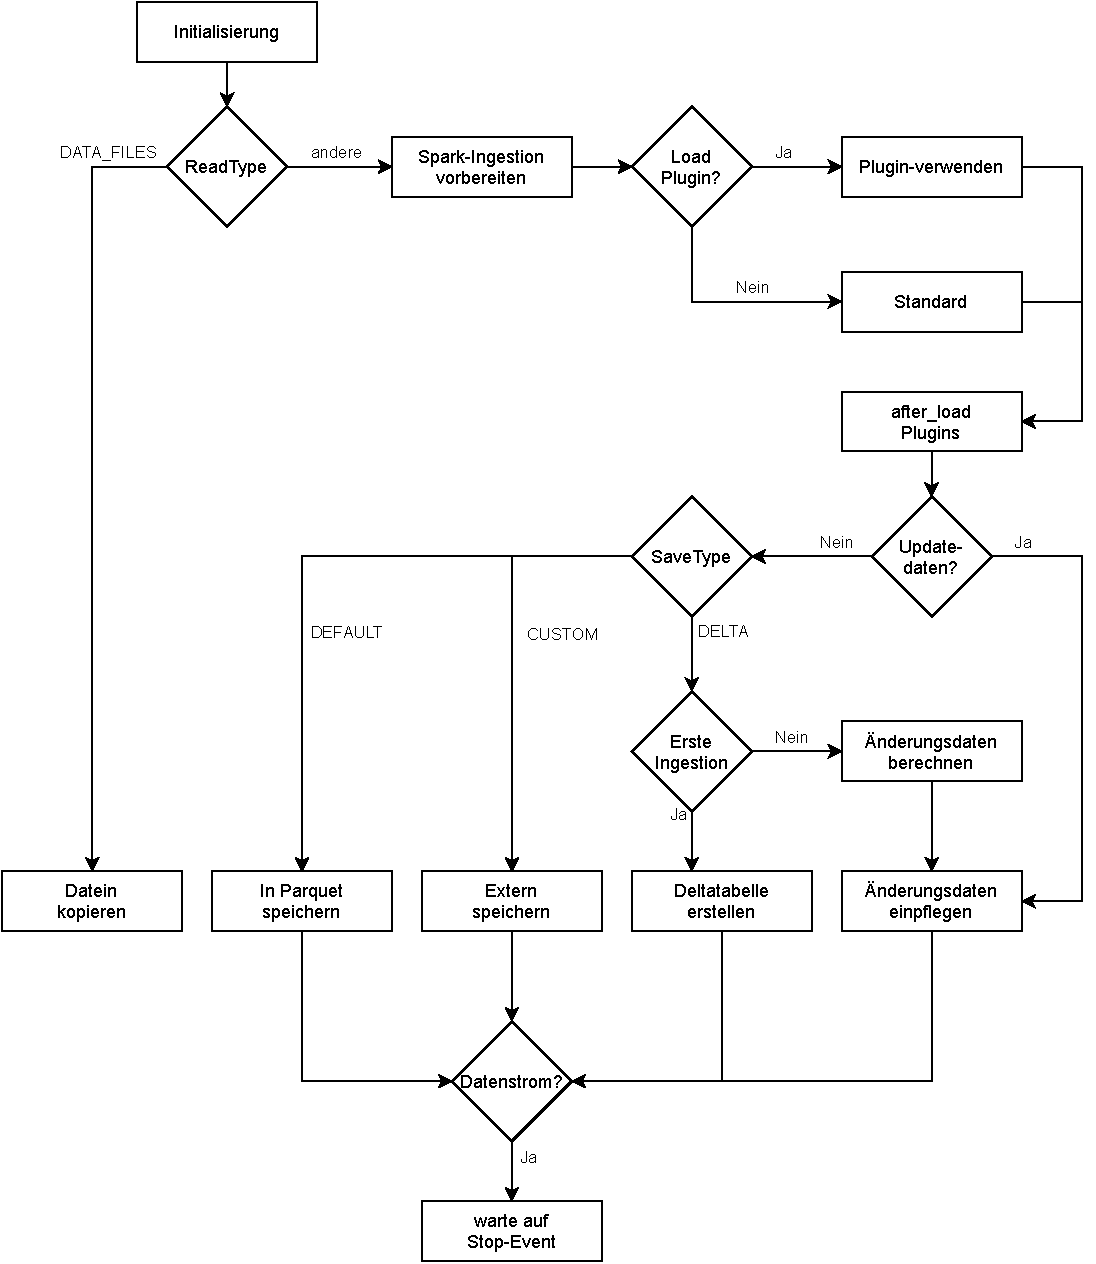
\includegraphics[width=\textwidth]{Grafiken/Umsetzung-Ingestion-Ablauf.pdf}
    \caption{Ablauf einer Ingestion}
    \label{fig:umsetz-ingestion-ablauf}
\end{figure}